\documentclass{report}

%\usepackage{times}
\usepackage[pdftex,
  colorlinks=true,
  pdfstartview=FitV,
  linkcolor=blue,
  citecolor=blue,
  urlcolor=blue]{hyperref}
\usepackage{geometry}
\geometry{a4paper}
\usepackage{amssymb}
%\usepackage{epstopdf}
\usepackage{xspace}
\usepackage{indentfirst}

\usepackage[francais]{babel}
\usepackage[latin1]{inputenc}
\usepackage[dvips]{graphicx}
\usepackage{array}
\usepackage{multirow}
\usepackage{fancyheadings}
\usepackage[Lenny]{fncychap}
\pagestyle{fancy}
\newcommand{\sauteligne}{\vspace{0.5cm}}
\newcommand{\visidia}{ViSiDiA\xspace}
\newcommand{\berlios}{BerliOs.de\xspace}
\author{}
\date{}

\title{
  \begin{flushright}
    \begin{Huge}
      \begin{textbf}
        Projet \visidia\\
      \end{textbf}
    \end{Huge}
    \rule{\textwidth}{2mm}\\
    \large\rm{Cahier des charges}\\
    \vspace{2cm}
    \begin{textbf}\\
      \underline{Auteurs} :\\
      \vspace{0.5cm}
      \sc Nada Ayad\\
      Damien Cassou\\
      Xavier Durand\\
      Jean-Baptiste Gautron\\
      Hicham Ghriss\\
      Mathieu Hopmann\\
      Julie Quagliozzi\\
      \vspace{5mm}
    \end{textbf}
    \rm 10 f�vrier 2006
  \end{flushright}
}

\begin{document}
\maketitle
\tableofcontents

\chapter*{Introduction}
%          * D�crire la probl�matique et la motivation
%          * Placer le syst�me dans son contexte
%          * Donner son r�le dans l'organisation qui l'englobe 


\subsection*{Contexte d'utilisation}

L'algorithmique distribu�e devient de nos jours de plus en plus
importante aux vues des utilisations possibles sur les r�seaux et
autres syst�mes distribu�s.%\\

Cependant,  les   applications  distribu�es  qui   en  d�coulent  sont
difficiles � implanter, tester  et exp�rimenter.  En effet, celles-ci,
en  plus  des  probl�mes  des  applications  classiques  centralis�es,
doivent  g�rer  des probl�mes  de communication  entre processus,  de
concurrence  et de  conflits  de  ressources.  C'est  dans  le but  de
faciliter la t�che � un d�veloppeur d'algorithmes  distribu�s que des
chercheurs  du  LaBRI  ont   cr��  \visidia.%\\

Ce logiciel est un atelier proposant des outils
de simulation  et  de visualisation,  au travers  d'animations 
graphiques en temps r�el, de l'ex�cution d'un algorithme distribu� sur
un graphe  donn�.  Cet algorithme peut �tre  choisi dans une liste,
algorithme d�velopp� par  l'utilisateur ou encore  dessin� gr�ce � des
r�gles de r��criture.%\\ 

L'application  va  donc  constituer  �  terme un  outil permettant la 
validation pratique de r�sultats th�oriques sur un environnement
distribu�.
\subsection*{D�finition d'un r�seau}

Un r�seau est un graphe dont les sommets sont les processeurs et les
ar�tes sont les liens de communication.%\\  

\subsection*{Notions d'algorithmique distribu�e}

Il existe de nombreux mod�les permettant de d�crire des algorithmes
distribu�s. Parmi eux, deux ont �t� d�velopp�s dans \visidia : la
communication par 
�change de message et par agent.%\\ 

Dans la suite, nous parlerons de m�moire d'un agent et d'un sommet
mais la m�moire d'un sommet contient le whiteboard et l'�tat de ses
ports.%\\ 

\subsubsection*{Communication par message}

Dans ce mod�le, chaque n\oe ud repr�sente un syst�me ou un processeur. Sur chaque
n\oe ud est ex�cut� un algorithme disposant de certaines primitives qui lui permettent de
communiquer � l'aide de messages avec ses n\oe uds voisins.
Les n\oe uds sont reli�s entre eux par des canaux de communication
(les ar�tes du graphe) par lesquels transitent les messages. 

\subsubsection*{Communication par agent} (??? a modifier)

Ce second mod�le, plus r�cent que le pr�c�dent, consid�re que le syst�me
repr�sent� par un n\oe ud ne dispose pas d'unit� de calcul mais seulement d'une
m�moire. Les n\oe uds sont ainsi d�pourvu d'algorithme et ne peuvent donc pas
communiquer directement entre eux.%\\

L'ex�cution des algorithmes se fait par des agents. Ces entit�s poss�dent une
capacit� de calcul ainsi qu'une m�moire. Un agent se d�place dans le graphe
et ex�cute un algorithme qui lui est associ�.


\subsection*{L'existant}

\visidia impl�mente aujourd'hui les deux mod�les de communication pr�sent�s
pr�c�demment. La gestion des agents a �t� ajout�e l'ann�e derni�re. Seule cette
partie concernera le projet, la partie sur la communication par message ne sera
pas �tudi�e.%\\

L'application \visidia a �t� r�alis�e en respectant une s�paration en
trois parties, interface graphique, simulateur et algorithmes. 
L'interface graphique permet � l'utilisateur d'interagir avec le
programme et de consulter l'avancement d'une ex�cution d'agent sur un
graphe. Elle est synchronis�e avec le simulateur pour �viter toute
incoh�rence. Elle fournit quelques statistiques de base sur
l'ex�cution. Le simulateur coordonne les op�rations. C'est le c\oe ur
de \visidia. Enfin, ce sont les agents  qui vont r�aliser ces
op�rations sur le graphe.%\\ 

Une biblioth�que  de primitives de  base (\emph{API}) est mise �
disposition de l'utilisateur afin qu'il puisse r�aliser ses propres
algorithmes � base d'agent. 


\subsection*{Motivations et but}

La version avec agent mobile de \visidia offre aujourd'hui suffisamment de
fonctionnalit�s pour simuler les algorithmes � base d'agent mobile.%\\

N�anmoins, contrairement � la partie de \visidia avec communication par message
qui poss�de un grand nombre d'algorithmes d�velopp�s, la partie avec agent mobile
se limite � quelques-uns. L'impl�mentation des algorithmes dans \visidia n'est
pas ais�e et la proc�dure est peu document�e, le client a donc besoin
que les algorithmes soient impl�ment�s pour lui.%\\ 

Les statistiques sur l'ex�cution des algorithmes est un point particuli�rement
important pour le client. En effet, \visidia est un outil qui lui permet de
confronter r�sultats th�oriques et exp�rimentaux. C'est les statistiques qui
permettent cette comparaison et celles-ci sont actuellement tr�s limit�es.%\\

Un autre besoin du client est de pouvoir agir sur le graphe au cours de
l'ex�cution d'un algorithme. En effet, en algorithmique distribu�e on
s'int�resse aux cons�quences d'une �volution de la topologie du r�seau, de
l'alt�ration des m�moires d'un n\oe ud du r�seau ou d'un agent, voire du crash
accidentel d'un de ces derniers.

\chapter{Mod�le du syst�me}



\section{Cas d'utilisation}




\section{Diagramme de classes}

\begin{figure}
  \centering
  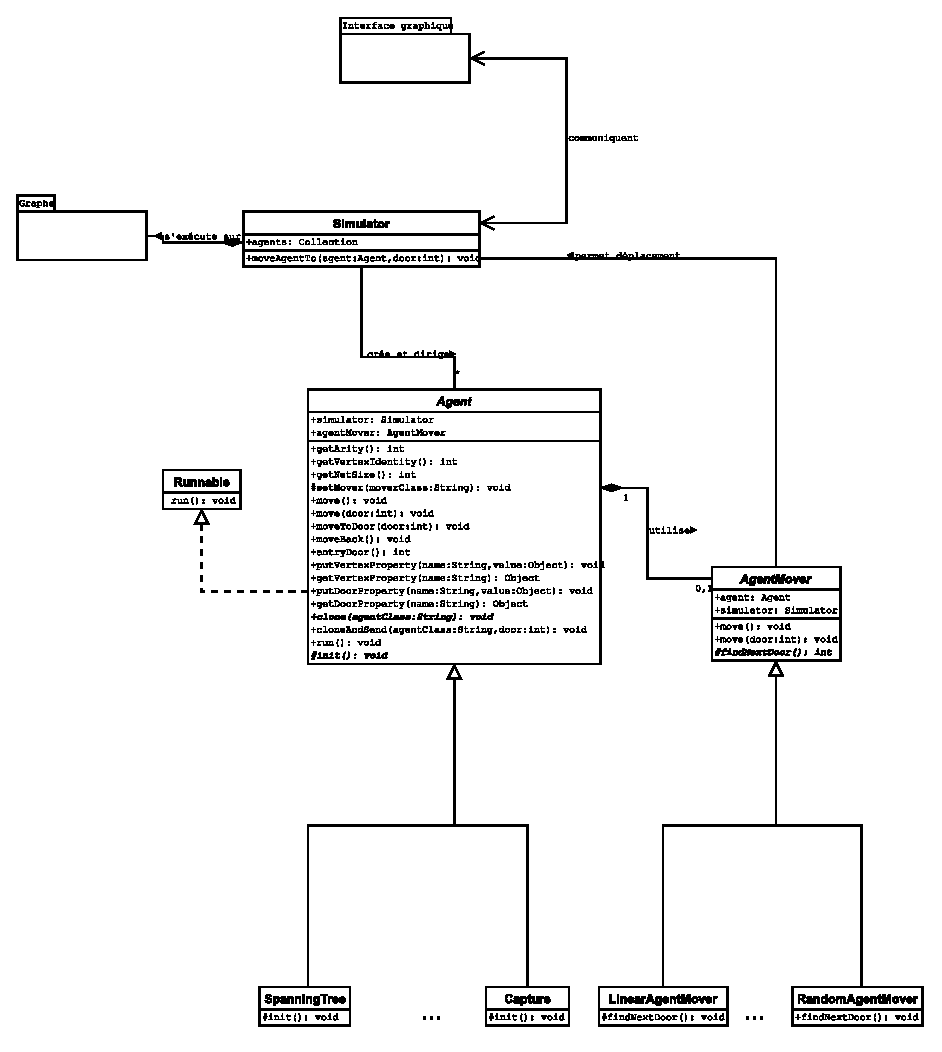
\includegraphics[width=15cm]{figures/classes}  
  \caption{Diagramme de classes}
\end{figure}


%% Local Variables:
%% mode: latex
%% coding: latin-1
%% TeX-master: "main"
%% End:
\chapter{Besoins fonctionnels et non fonctionnels}

Dans  cette partie  nous d�crirons  les besoins  fonctionnels  li�s au
projet  (A.P.I,  interface) ainsi  que  les  besoins non  fonctionnels
(langage, licence, etc).


\section{Description de l'A.P.I}
\label{sec:api}

Les m�thodes de la classe \emph{Agent} fournies � l'utilisateur pour
l'�criture de l'algorithme sont les suivantes :\\

\begin{description}

\item[getArity]  retourne  le nombre  de  portes  sortantes du  sommet
  courant (la premi�re est num�rot�e 0)
\item[getVertexIdentity] retourne le num�ro du sommet courant (suppose
  que l'algorithme utilise un identifiant unique pour chaque sommet)
\item[getNetSize] retourne le nombre de sommets du graphe
\item[setMover]  permet de  d�finir pour  l'agent un  nouveau  type de
d�placement dont le nom est pass� en param�tre
\item[move] permet de d�placer l'agent sur la porte suivante ou sur la
  porte dont le num�ro est pass� en param�tre
\item[moveBack] permet de d�placer l'agent sur la porte dont il vient
\item[entryDoor] retourne  le num�ro de la porte  par laquelle l'agent
  vient d'arriver
\item[putVertexProperty] place une propri�t� sur le sommet courant, la
  valeur et la cl� sont pass�es en param�tre
\item[getVertexProperty] retourne  la valeur  de la propri�t�  dont la
  cl� est pass�e en param�tre
\item[putDoorProperty] place une propri�t� sur une porte, le num�ro de
  la porte, la cl� et la valeur sont pass�s en param�tre
\item[getDoorProperty] retourne la valeur  de la propri�t� dont la cl�
  est pass�e en  param�tre, sur la porte dont  le num�ro est �galement
  pass� en param�tre
\item[clone] clone l'agent en cours (avec son tableau blanc)
\item[cloneAndSend] clone l'agent en cours (avec son tableau blanc) et
  envoie le clone sur la porte pass�e en param�tre
\item[nextStep] bloque l'agent jusqu'� ce que tous les agents de notre
  graphe  aient appel�  cette  m�me m�thode.  Permet  un m�canisme  de
  synchronisation\\

\end{description}

Il sera ainsi possible de cloner un \emph{agent}, et �ventuellement de
l'envoyer sur  une porte. L'\emph{agent}, ainsi cr��,  pourra avoir un
type de d�placement, ainsi qu'un  algorithme diff�rents de ceux de son
p�re.\\

Les  \emph{agents}  auront  �galement  d'autres  fonctionnalit�s,  ils
doivent  notamment   pouvoir  se  rencontrer,   c'est-�-dire,  pouvoir
d�tecter qu'un  autre \emph{agent} est sur  le m�me sommet,  ou sur la
m�me ar�te. Cela  va imposer la mise en place  de r�gles de priorit�s,
pour que  plusieurs \emph{agents}  ne puissent pas  agir simultan�ment
sur un m�me sommet.\\

Enfin,  les agents  pourront, s'ils  le souhaitent,  faire appel  � un
syst�me de synchronisation afin d'effectuer des actions et se d�placer
de mani�re coordonn�e.\\

L'initialisation  des objets  se fera  au plus  tard. En  effet,  ils ne
seront initialis�s, que lorsqu'ils  seront utilis�s. Pour les tableaux
blancs des  sommets, notamment, leur  initialisation ne se  fera qu'au
passage d'un \emph{agent}, s'il celui-ci souhaite lire une valeur.

\section {Interface}

Notre  graphe  pourra d�buter  avec  autant  d'agent  que le  souhaite
l'utilisateur, tous les agents n'�tant pas forc�ment du m�me type.\\

L'utilisateur aura diff�rentes possibilit�s pour placer ses agents :\\

\begin{itemize}

\item \textbf{A la  souris : } L'utilisateur choisit  un type d'agent,
et le place  sur les sommets o� il souhaite  faire d�marrer les agents
de ce type.   Il peut ensuite choisir d'autres  types d'agent pour les
placer sur les sommets restants.\\

\item \textbf{Par fichier :  } L'utilisateur cr�e un fichier contenant
l'identifiant de chaque sommet o�  il souhaite voir d�marrer un agent,
auquel  il rattache  un type  d'agent.  Cela  revient au  m�me  que la
m�thode � la souris, mais est indispensable pour les graphes de grande
taille.\\

\item \textbf{Al�atoire  : } L'utilisateur choisit un  type d'agent et
une quantit� (1,2,...,*).  Le logiciel se charge alors  de r�partir ce
ou ces  agents de  fa�on al�atoire sur  les sommets du  graphe.  Cette
m�thode pourrait �tre int�ressante pour tester des algorithmes de type
policiers/voleur, avec plusieurs agents essayant d'en encercler un.

\end{itemize}

\section{Diagrammes de s�quences}

Nous d�crirons dans cette  section quelques sc�narios possibles durant
la vie d'un agent.

\subsection{D�placement}

Figure  \ref{fig:diagramme_seqDeplacement} :  Sc�nario  de d�placement
d'un agent sur le graphe.

\begin{figure}[h!t]
  \centering
  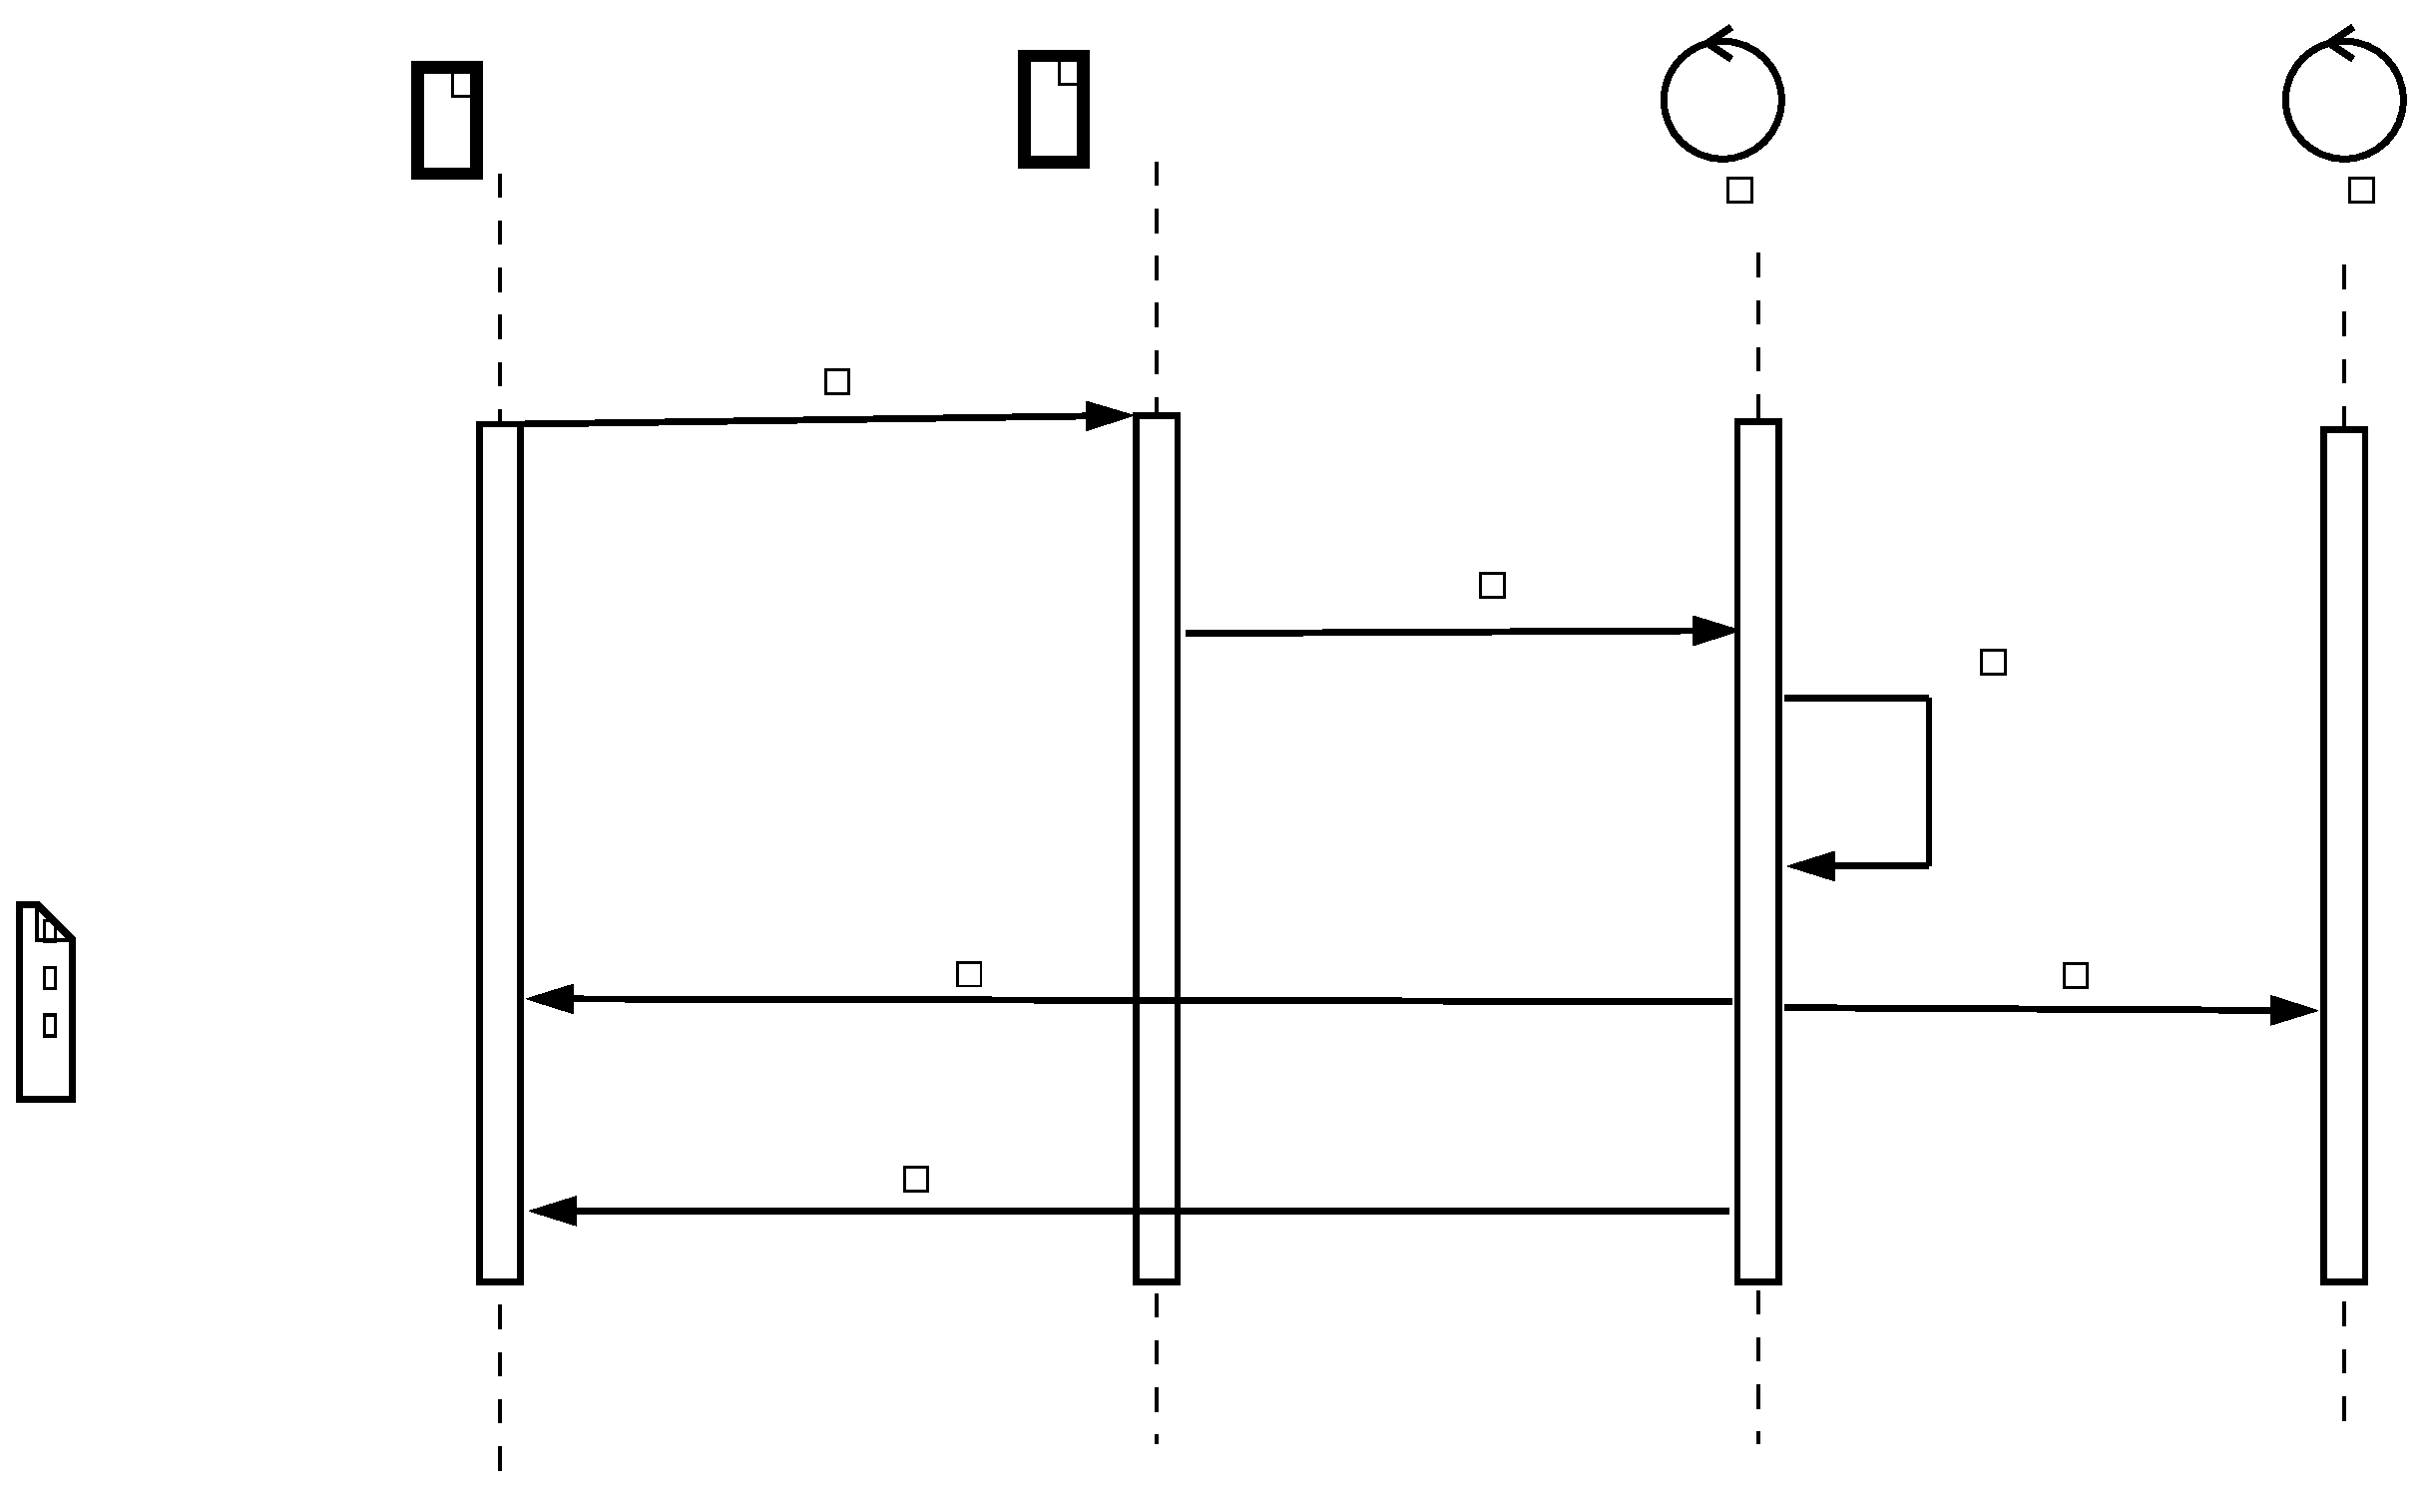
\includegraphics[width=14cm]{seqDeplacement}
  \caption{Sc�nario de d�placement}
  \label{fig:diagramme_seqDeplacement}
\end{figure}

\subsection{Propri�t�s}

Figure   \ref{fig:diagramme_seqProperties}  :   Sc�nario   o�  l'agent
souhaite modifier ou obtenir une propri�t� d'un sommet.

\begin{figure}[h!t]
  \centering
  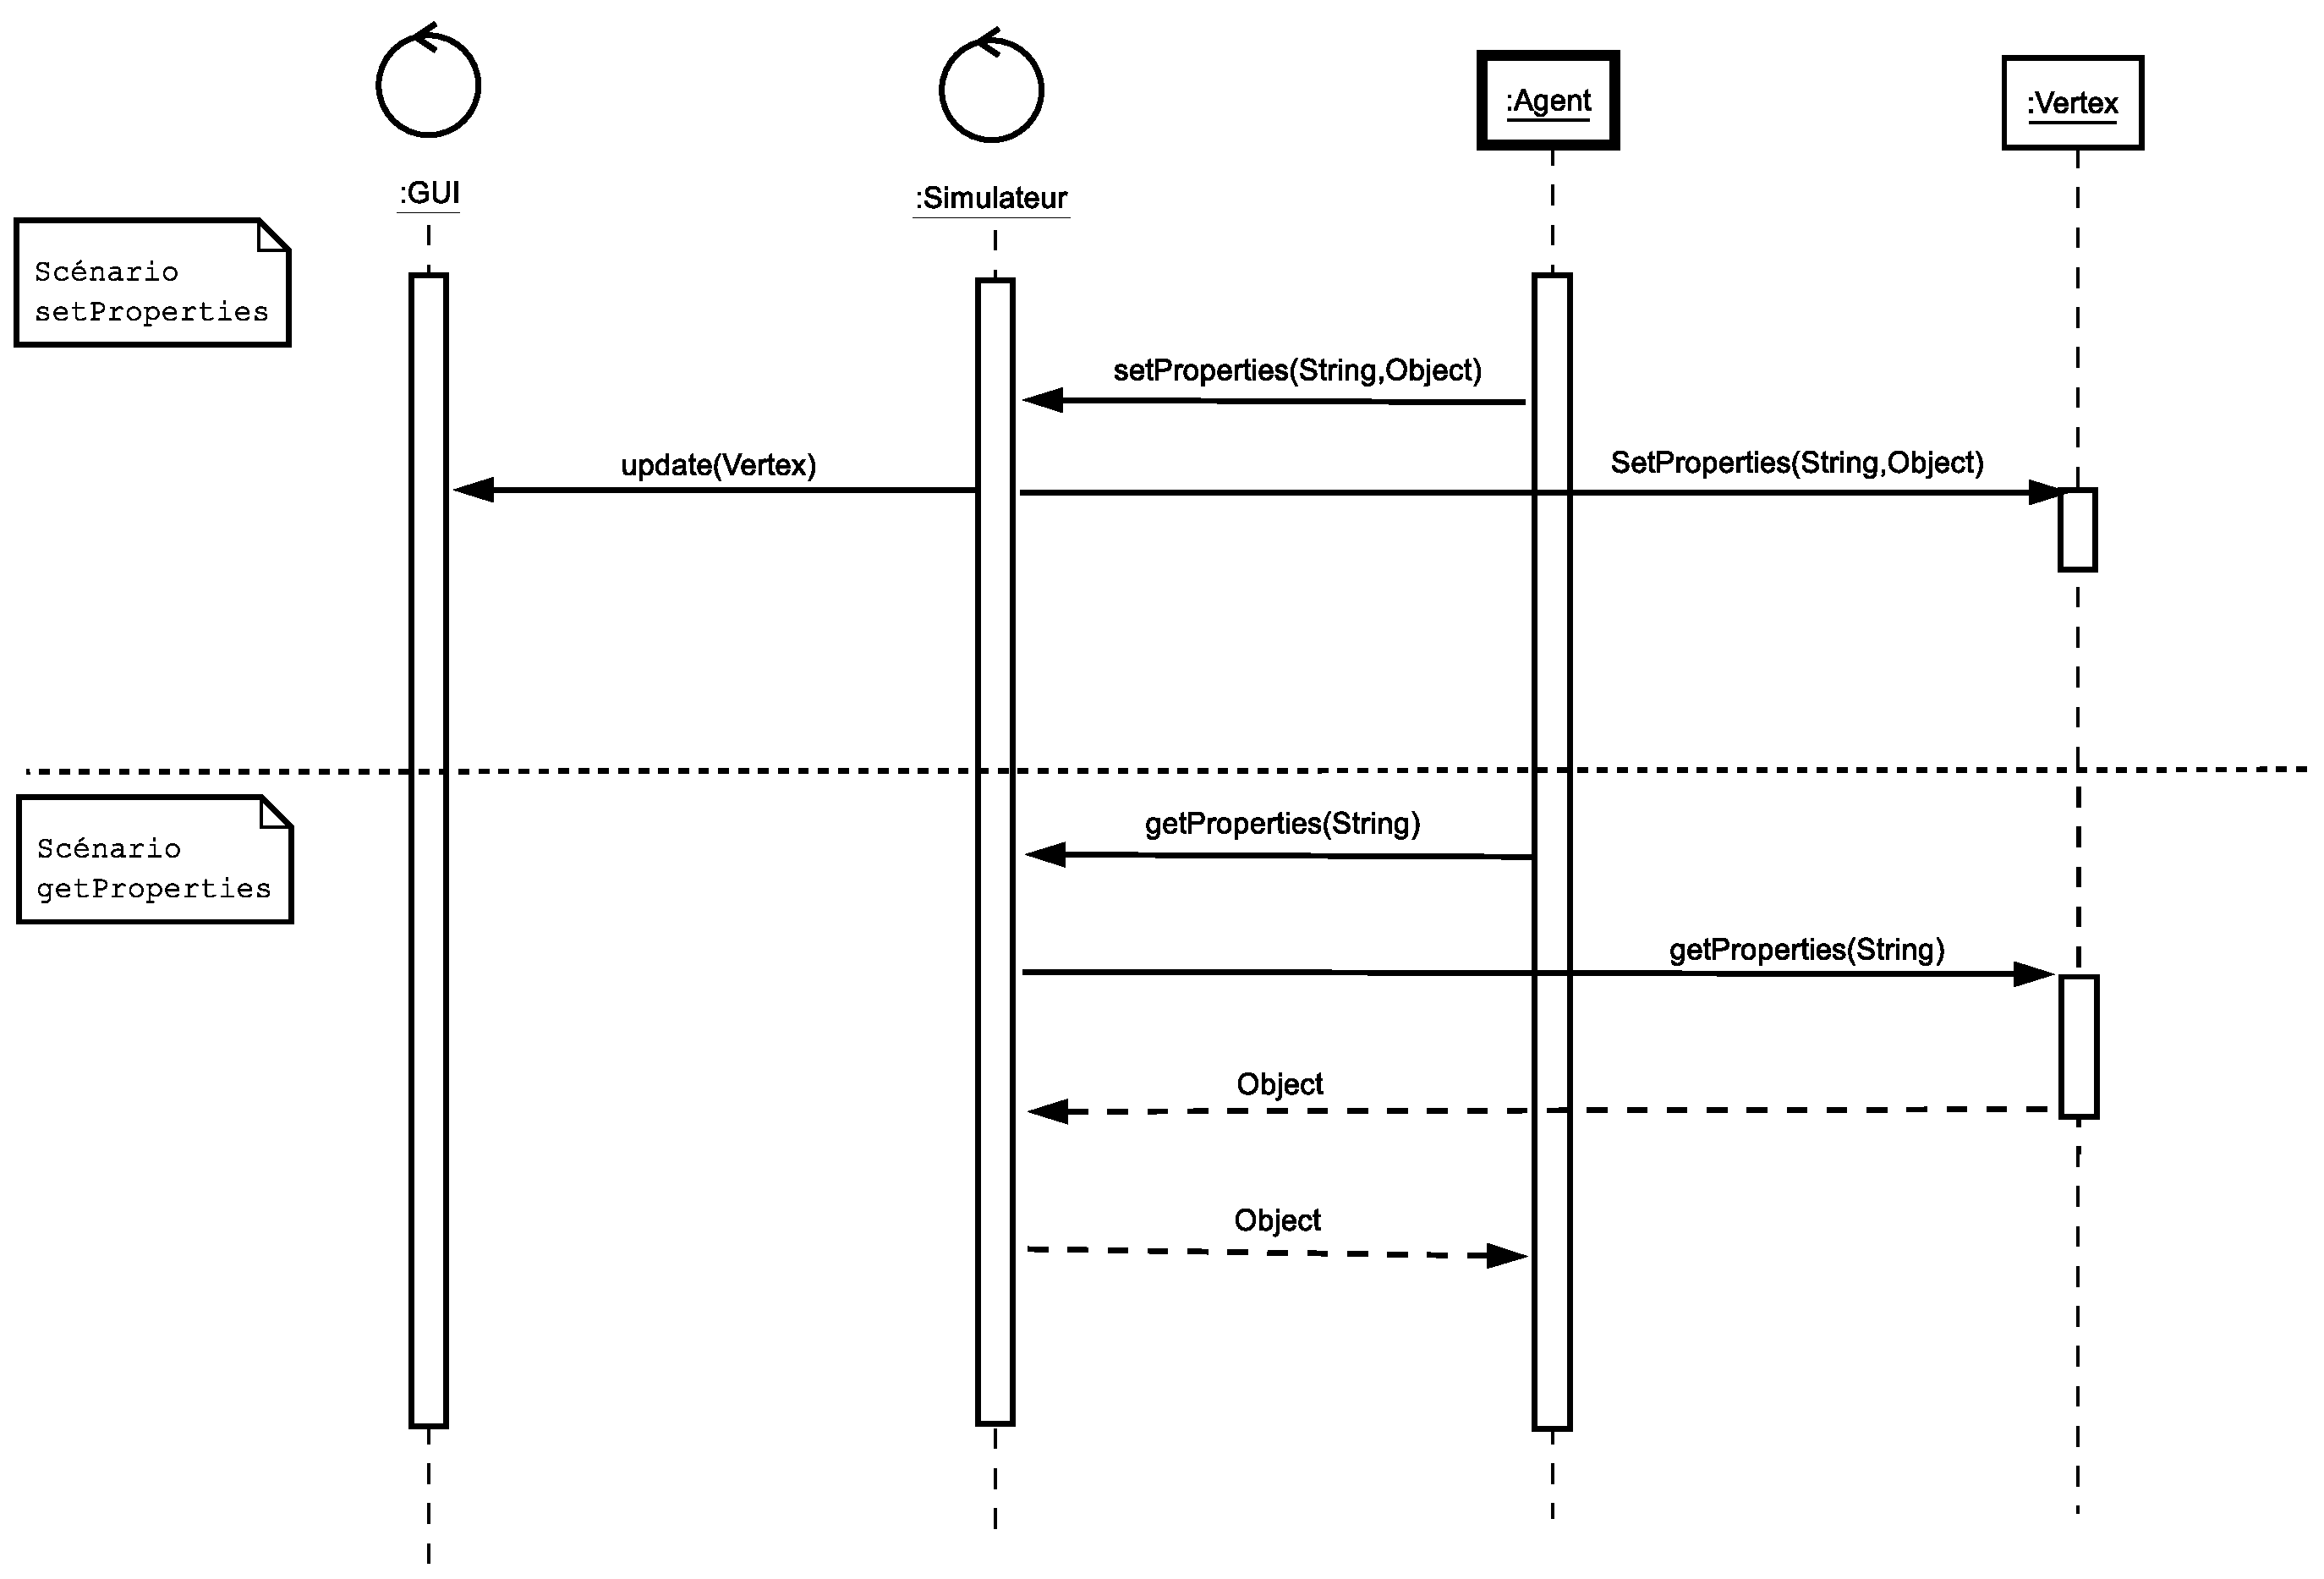
\includegraphics[width=14cm]{seqProperties}
  \caption{Sc�nario de lecture ou �criture d'une propri�t�}
  \label{fig:diagramme_seqProperties}
\end{figure}



\section{Contraintes}

\subsection{Langage et portabilit�}

Notre r�le  est de  d�velopper une extension  de \visidia, �crit  � la
base en  Java :  c'est donc  en Java que  nous �crirons  l'ensemble de
notre  programme,   afin  que  notre  module  s'int�gre   au  mieux  �
l'application.\\

Les  d�veloppeurs ext�rieurs seront  oblig�s de  passer par  notre API
pour concevoir de nouveaux  algorithmes distribu�s, ce qui nous impose
d'�tre compris le plus ais�ment possible par tout le monde. Pour cette
raison,  notre code  sera  r�dig� exclusivement  en  anglais. Le  Java
semble encore un  choix correspondant � notre volont�,  d'une part car
il  s'agit d'un  des langages  les plus  utilis�s actuellement  (si ce
n'est  LE plus  utilis�), d'autre  part  pour sa  portabilit� sur  les
diff�rentes plateformes existantes.\\

La  documentation quant  �  elle  sera r�alis�e  �  l'aide de  l'outil
Javadoc.\\


\subsection{Standard de codage}

*Utilisation des conventions JAVA :
\begin{itemize}
\item noms des classes commencant par une majuscule
\item noms des m�thodes commencent par une minuscule
\item majuscules pour separer les differents mots composant un nom 
\item accesseurs commen�ant par 'get'
\item modificateur commencant par 'set'\\
\end{itemize}

*Autres standards
\begin{itemize}
\item nom des classes et des methodes en anglais
\item reprise au maximum des noms existant
\item utilisation de noms explicites
\item commentaires en anglais style Javadoc
\end{itemize}

\subsection{Licence} 

L'ensemble de notre  programme sera sous licence GNU  GPL (GNU General
Public License)  version 2  ou sup�rieure. Une  version de  la licence
sera disponible en  fran�ais et en anglais dans le  code source, et un
rappel sera effectu� � chaque en-t�te de fichier.


%% Local Variables:
%% mode: latex
%% coding: latin-1
%% TeX-master: "main"
%% End:
\chapter{Organisation}

\section{Planning des taches}

%%   - Diagramme de Gantt si possible
%%   ;;planning des rendez-vous
%%   - planning des �tapes de remise du projet

\begin{figure}[p]
  \centering
  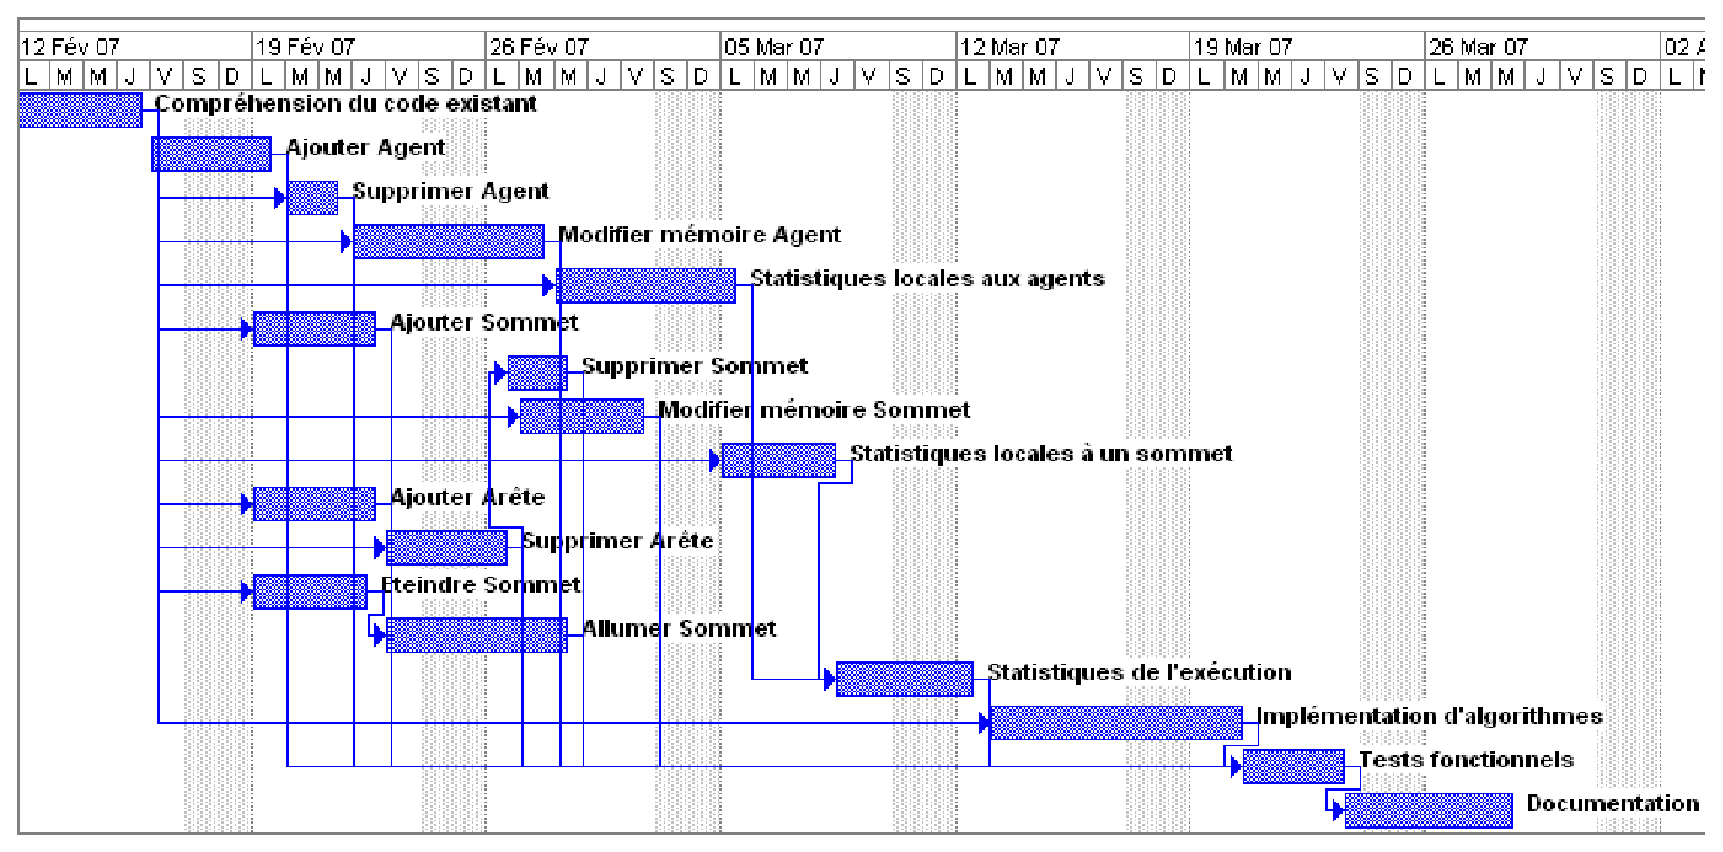
\includegraphics[angle=90,scale=0.8]{gantt}
  %\includegraphics[scale=0.8]{visidia.gantt}
  \caption{Diagramme de Gantt}
  \label{fig:gantt}
\end{figure}


L'�quipe  des r�alisateurs rencontrera  les clients  une fois  par semaine
pour faire le point sur le travail effectu�. L'horaire du vendredi matin �
10h  a �t� retenu  pour cette  entrevue hebdomadaire.  Les clients  et les
r�alisateurs resteront  en contact et  pourront �changer sur le  projet au
moyen d'une liste de diffusion \ref{mailing-list}.

Un diagramme  de Gantt \ref{fig:gantt}  planifie les grandes �tapes  de la
r�alisation du projet. Ce diagramme sera mis � jour au cours de la vie du projet.

\section{�ch�ancier}

La date de remise des rapports de fin de PFA aux clients est fix�e au
vendredi 14 avril, 17h00 derni�re limite.

La remise du projet donnera lieu � une soutenance dont la date est
fix�e au jeudi 27 avril.

%\section{Description des outils}
%% - D�ploiement (cd,dvd,autre)
%% - Presentation du portail, du site, de la mailing liste, etc.
%% - methode de validation du travail (tests, iteratif ou unitaire)

%\section{Utilisation d'une plate-forme de d�veloppement}
\section{Plate-forme de d�veloppement}

Le projet sera l'occasion d'utiliser un portail �volu� de
d�veloppement sur le mod�le du c�l�bre portail
%\href{http://sourceforge.net}{SourceForge}.
%\url{http://sourceforge.net} 
SourceForge \cite{SourceForge}.
Notre choix s'est port� sur le portail
%\href{http://www.berlios.de}{\berlios}
%\url{http://www.berlios.de} 
\berlios \cite{BerliOs} pour des raisons de rapidit� des
serveurs. Notre projet \visidia dispose ainsi d'une page d'accueil \cite{visidiaPFA}.\\
\url{http://visidia.berlios.de}\\
%\href{http://visidia.berlios.de}{\visidia.\berlios} 

%% \begin{verbatim}
%% http://visidia.berlios.de
%% \end{verbatim}

Cette page  d'accueil est un  wiki \cite{wiki}. Cela permet  une �volution
plus souple des informations pr�sent�es. Cette page est le point de d�part
vers  les  diff�rents services  fournis  par  \berlios.  Tous les  modules
d�crits par la suite peuvent �tre  retrouv�s � partir de la page d'accueil
du projet.\\

Tout d'abord les sources de notre extension de \visidia sont
maintenues gr�ce au gestionnaire de version Subversion
\cite{subversion}. Le client a la possibilit� de suivre l'avanc�e du
projet en acc�dant aux sources. Deux interfaces web permettent l'acc�s
aux sources: viewcvs \cite{viewcvs} et websvn \cite{websvn}.\\ 
%\href{http://svn.berlios.de/viewcvs/visidia/}{viewcvs}
\url{http://svn.berlios.de/viewcvs/visidia/}\\
%\href{http://svn.berlios.de/wsvn/visidia/}{websvn}
\url{http://svn.berlios.de/wsvn/visidia/}\\ 

Il est �galement possible de t�l�charger anonymement les sources
depuis le d�p�t Subversion:
\begin{verbatim}
svn checkout svn://svn.berlios.de/visidia/trunk
\end{verbatim}

L'�quipe  a aussi mis  en place  des mailing-lists  g�r�es par  le portail
\berlios.   Une  mailing-list  permet  aux  clients de  joindre  tous  les
r�alisateurs  et vice  versa. L'adresse  de cette  liste de  diffusion est
%\url{mailto:visidia-pfa@berlios.de}
\label{mailing-list}:
\begin{verbatim}
visidia-pfa@berlios.de
\end{verbatim}

Il est possible  de consulter les archives de cette  liste de diffusion au
moyen d'une interface web \cite{mailing-list}.\\
\url{https://lists.berlios.de/mailman/private/visidia-pfa/} 
 

%% Local Variables:
%% mode: latex
%% coding: latin-1
%% TeX-master: "main"
%% End:
\chapter{Lexique}

Vous  trouverez  ci-dessous les  d�finitions  relatives aux  principaux
termes et sigles utilis�s dans la r�alisation du cahier des charges.


\begin{description}

\item[Algorithmique distribu�e] : cette partie de l'algorithmique
s'int�resse aux algorithmes s'ex�cutant sur plusieurs unit�s de calcul
en m�me temps. Le mod�le th�orique d'un r�seau dans ce cadre est un
graphe dont les sommets (ou noeuds) sont des machines ou processeurs
et les ar�tes des connexions.

\item[Agent   mobile]   :   entit�   autonome   de   calcul   qui   se
d�place \cite{agentBook}.

\item[A.P.I.]   :  Application  Programming  Interface.   Ensemble  de
prototypes   de  fonctions   accessibles   depuis  l'ext�rieur   d'une
biblioth�que. C'est l'interface publique de la biblioth�que.

\item[GUI]  :  Graphical  User  Interface. Interface  qui  permet  une
  utilisation  simple  d'un  programme  : elle  int�gre  notamment  un
  environnement graphique et permet l'utilisation de la souris.

\item[Javadoc] :  outil qui  permet de g�n�rer  de la  documentation �
  partir du code source et des commentaires Java.

\item[R�gle  de  r��criture] :  r�gle  de  transformation locale  d'un
  graphe.  L'application d'une telle  r�gle entra�ne le changement, en
  fonction de  voisins, des  �tats des sommets  et des ar�tes  dont la
  configuration correspond aux conditions d'application de la r�gle.

\item[Thread  ou processus  l�ger]  :  un thread  est  similaire �  un
  processus : il ex�cute  un ensemble d'instructions. Toutefois, l� ou
  chaque processus  poss�de sa  propre m�moire virtuelle,  les threads
  qui appartiennent au m�me processus p�re partagent un m�me partie de
  sa m�moire virtuelle.

\item[\visidia]   :  Visualization   and  Simulation   of  Distributed
Algorithms  ou Visualisation  et  Simulation d'Algorithmes  Distribu�s
\cite{visidiaLaBRI}.

\end{description}



%% Local Variables:
%% mode: latex
%% coding: latin-1
%% TeX-master: "main"
%% End:

\bibliographystyle{plain}
\bibliography{myBib}

%% Local Variables:
%% mode: latex
%% coding: latin-1
%% TeX-master: "main"
%% End:


\end{document}

%% Local Variables: 
%% mode: latex
%% TeX-master: t
%% coding: latin-1
%% End: 
